\documentclass[10pt,a4paper]{article}
\usepackage[margin=2cm]{geometry}
\usepackage{graphicx,booktabs,amsmath,amssymb,hyperref,enumitem,float}
\setlist{nosep,leftmargin=*}
\setlength{\parskip}{4pt}\setlength{\parindent}{0pt}
\title{AI651 Deep Learning for Space, Time and Graphs\\Programming Assignment 1}
\author{Ahmed Jawed}
\date{October 2026}
\begin{document}
\maketitle
\begin{center}
\textbf{Code repository:} \url{https://github.com/ahmedjawedaj/DL4STG-PA1}
\end{center}

\noindent\textbf{Contents.} Task 1 (implementation, five responses, figures from the
\texttt{PA1\_PRESET=full} run). Task 2 (Autoformer pipeline, validation, required
optional-data ablation, submission). Generative-AI disclosure at the end.

% ---------------------------------------------------------------------------
% Task 1 responses. All numbers come from the PA1_PRESET=full run
% (data seed 0, model seed 0, CPU). Tables: results/design/<output>.csv
% Populations: "established" = stations 1-3, "held-out" = station 4.
% Split named in every claim: validation = targets in [9600, 12480).
% ---------------------------------------------------------------------------
\section{Task 1: Forecasting Across Heterogeneous Sensors}

\subsection*{Implementation summary}
\begin{itemize}
  \item \texttt{RawAttentionForecaster.forward}: circular Conv1d embedding of the
        $[B,1,L]$ context, add the learned position table, two encoder blocks, final
        LayerNorm, flatten $[B,L\cdot d]$ and a linear head to $[B,H]$.
  \item \texttt{SeriesDecomposition.forward}: replicate the first and last sample
        $\lfloor m/2\rfloor$ times, \texttt{avg\_pool1d} with stride 1 along time, return
        $(x-T,\,T)$ so that $S+T=x$ exactly.
  \item \texttt{aggregate\_delays}: build the source index $(t-\tau_j)\bmod L$ for every
        example and selected delay, \texttt{gather} the shifted values, weight and sum over
        $j$. Fully vectorised and differentiable in values and weights.
\end{itemize}
All notebook checks pass, including the worked decomposition and delay-aggregation examples.

% ---------------------------------------------------------------------------
\subsection*{Response 1A: expected versus measured ordering (Output 1.1)}

\textbf{Expected ordering, written before Output 1.1.}
Established stations: period-routed ridge $<$ Raw Attention $<$ sensor-specific ridge
$\approx$ shared ridge (RMSE). Held-out station 4: the same, with sensor-specific ridge
unavailable and every model slightly worse than on stations 1--3.

\textbf{Measured (validation, RMSE in m/s$^2$).}

\begin{center}\small
\begin{tabular}{lcccc}
\toprule
Model & Established & Held-out 4 & Params & Fit (s)\\
\midrule
Shared ridge          & 0.767 & 0.876 & 4\,608 & 0.01\\
Sensor-specific ridge & 0.768 & n/a   & 13\,824 & 0.09\\
Period-routed ridge   & \textbf{0.166} & \textbf{0.173} & 59\,904 & 0.03\\
Raw Attention         & 0.426 & 0.607 & 368\,368 & 928\\
\bottomrule
\end{tabular}
\end{center}

\begin{itemize}
  \item \textbf{Ordering held}: routed ridge $<$ Raw Attention $<$ shared $\approx$
        sensor-specific on both populations and in every product.
  \item \textbf{Size of the gaps}: routing cuts shared-ridge RMSE by 78\% on stations
        1--3 (0.767 to 0.166). Raw Attention recovers only about 57\% of that gain
        (0.426) with 6$\times$ the parameters of the routed ridge.
  \item \textbf{Sensor identity adds nothing}: sensor-specific ridge is 0.768 against
        0.767 for shared. Per-product RMSEs match to within 0.01 (A 0.804 vs 0.805,
        C 0.630 vs 0.621). Station identity is not the variable that changes the rule.
  \item \textbf{Across products}: shared ridge is worst on Product B (0.854) and best on
        C (0.621). Routed ridge is flat across products (0.181, 0.164, 0.152).
  \item \textbf{Held-out station}: routed ridge barely moves (0.166 to 0.173, +4\%).
        Raw Attention degrades by 42\% (0.426 to 0.607). A plausible (untested)
        explanation is that its learned mixing partly fits the amplitude, mounting phase
        and drift of the three fitted stations.
  \item \textbf{Revision}: I expected Raw Attention to be closer to the routed ridge.
        The explicit pace variable is worth more than generic context-dependent mixing
        in this world, and it transfers to an unseen sensor because pace is shared by
        the whole line while sensor details are not.
\end{itemize}

% ---------------------------------------------------------------------------
\begin{figure}[h]\centering
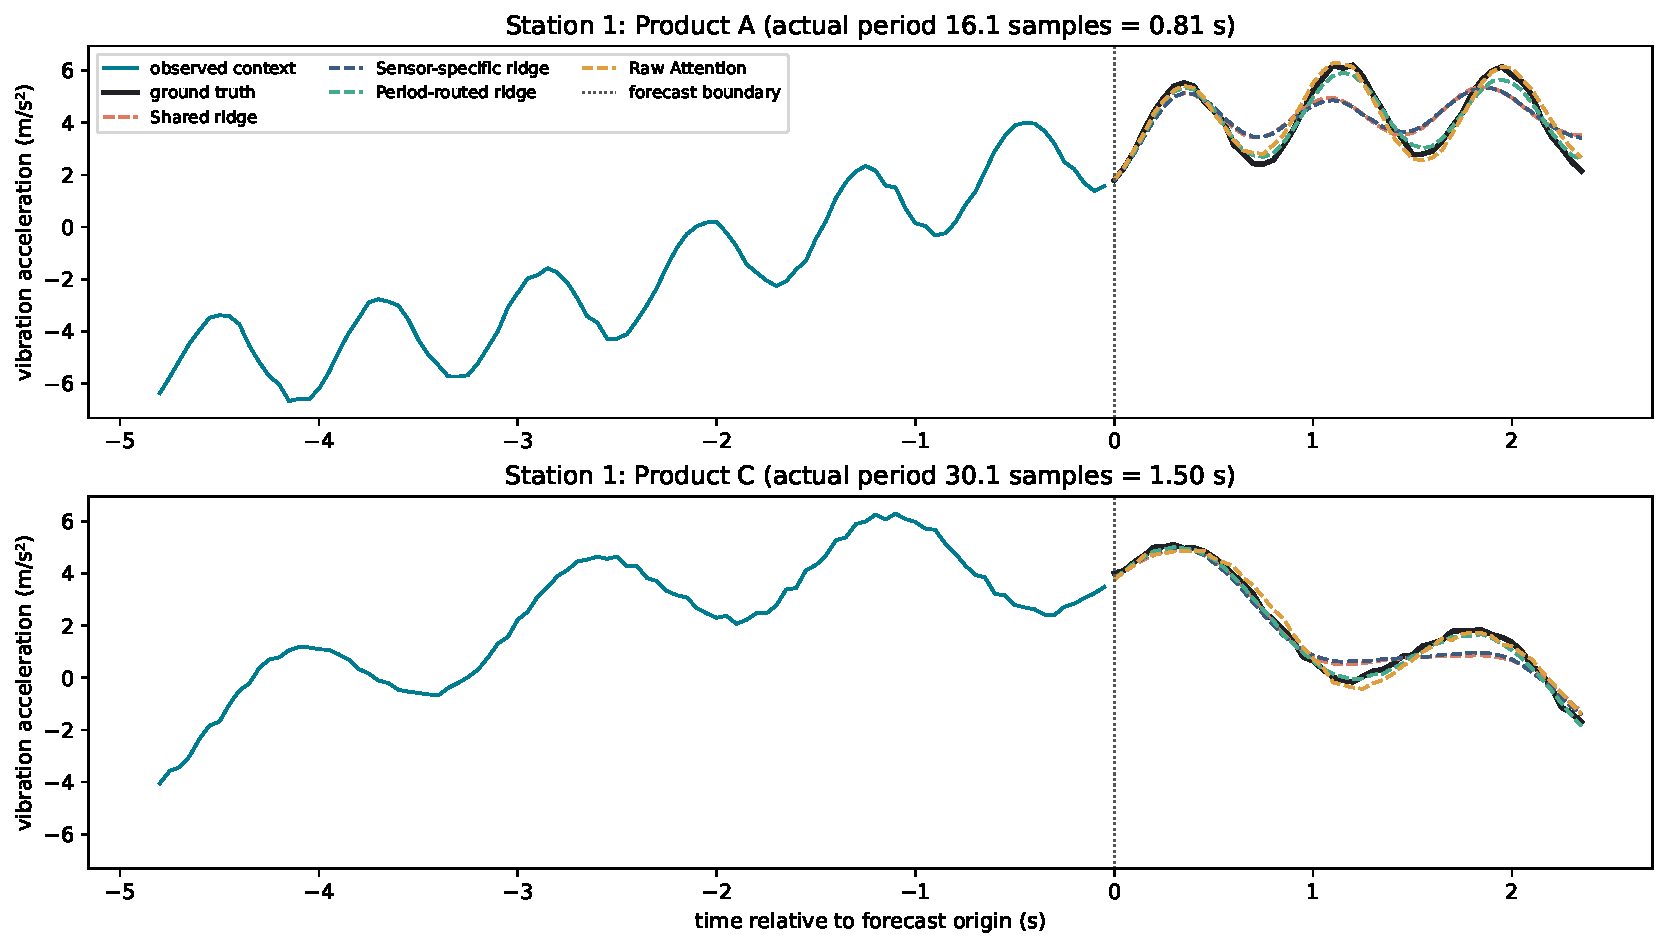
\includegraphics[width=0.49\linewidth]{figures/1.2-1.pdf}\hfill
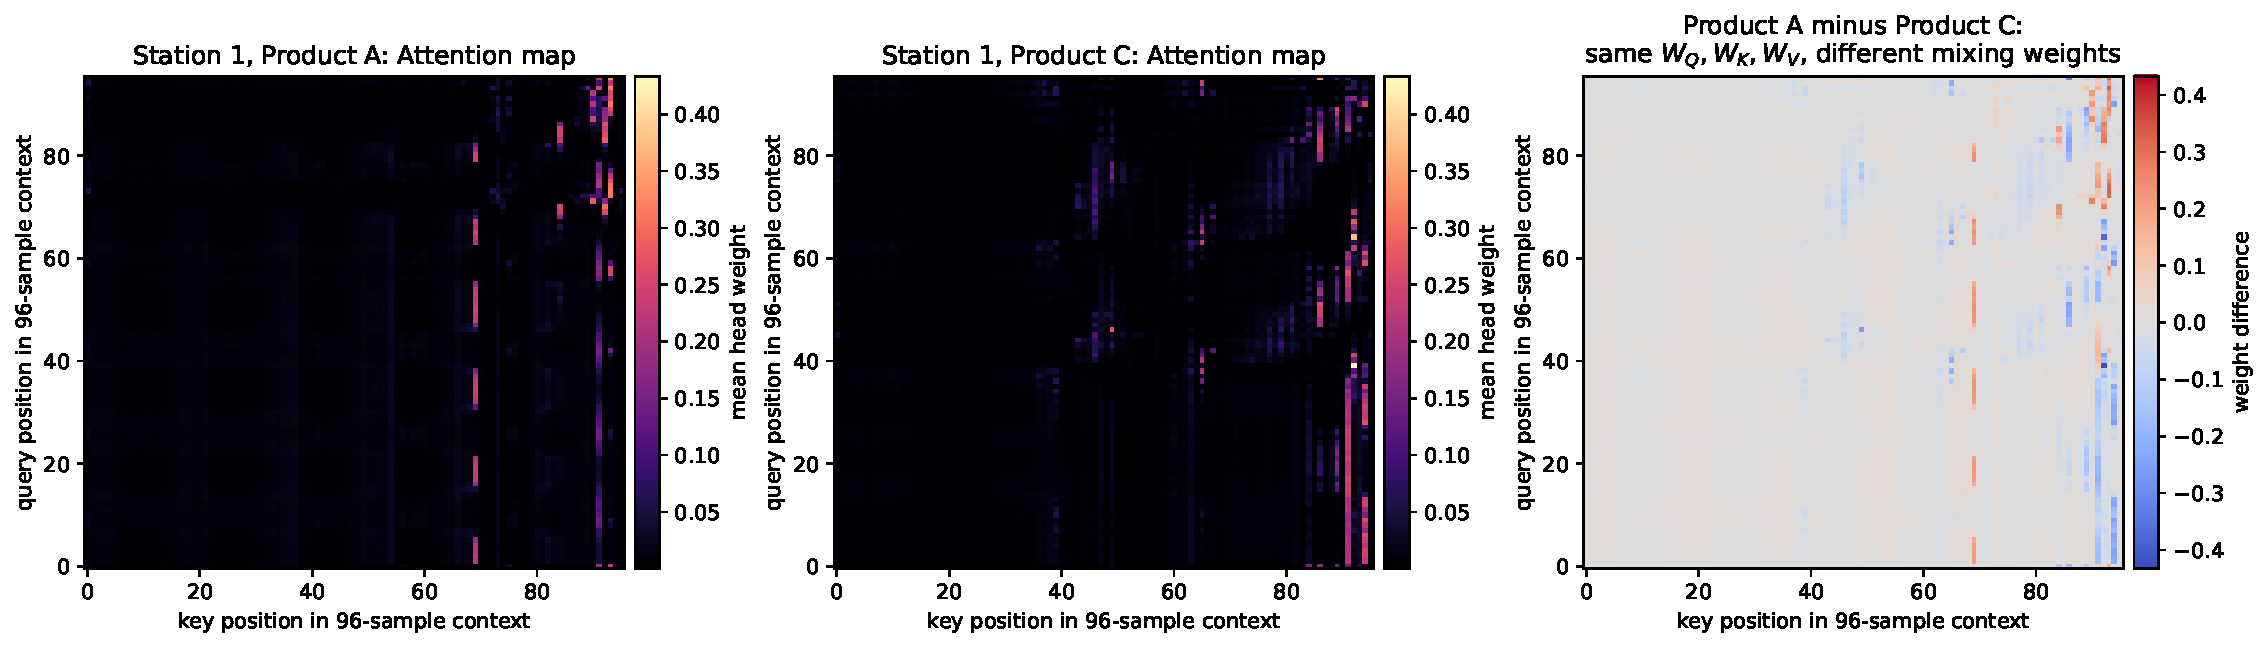
\includegraphics[width=0.49\linewidth]{figures/1.3-1.pdf}
\caption{Output 1.2 (left): station 1 under Products A and C. Output 1.3 (right): Attention maps for the two contexts and their difference.}\label{fig:o12}
\end{figure}

\subsection*{Response 1B: why the rule must depend on context (Outputs 1.2, 1.3)}

\begin{itemize}
  \item \textbf{The compromise in Output 1.2 (validation windows).} On station 1,
        Product A (period 16.1), shared and sensor-specific ridge produce a damped
        oscillation: amplitude is roughly halved and the peaks drift slightly out of phase
        with the truth (window RMSE 0.779 and 0.787). On Product C
        (period 30.1) the same matrix fits much better (0.448 and 0.436).
  \item \textbf{Why.} $\widehat{W}$ in Eq.~(8) is one fixed linear map. Continuing a
        cycle of period 16 and one of period 30 requires different phase advances from
        the same lags. Least squares averages over all training paces. Continuations
        that disagree in phase partly cancel, so the forecast shrinks in amplitude and its
        phase is only approximately right. The damping is the visible cost of averaging
        incompatible continuations.
  \item \textbf{Routed ridge avoids it} because each pace band has its own
        $\widehat{W}$ (0.232 and 0.150 on the same windows). Raw Attention also tracks
        both (0.287 and 0.270) without being told the pace.
  \item \textbf{How Attention changes the operator (Output 1.3, validation windows).} $W_Q, W_K, W_V$ are
        the same for both windows. The weights $\mathrm{softmax}(QK^\top/\sqrt{d_h})$
        are recomputed from each window, so the mixing matrix differs: mean absolute
        difference 0.011 per entry but up to 0.433 on individual query and key pairs.
        The Product A map concentrates on a few key columns late in the context, the
        Product C map spreads over bands near positions 40 to 95.
  \item \textbf{Contrast.} Ridge applies $\hat z = x^\top\widehat{W}$ with the same
        $\widehat{W}$ for every context. Attention applies $\hat z = f(A(x)\,V(x))$ where
        $A(x)$ is built from the input. Output 1.3 shows only that the mixing depends on
        the context, not that it has recovered the physical period.
\end{itemize}

% ---------------------------------------------------------------------------
\subsection*{Response 2: separating slow structure from repetition (Outputs 2.1--2.3)}

\begin{itemize}
  \item \textbf{Selected width: $m=41$}, chosen by the harness on training windows of
        stations 1--3 via the oracle recovery score (Output 2.2: raw 0.687, widths
        17/25/33/41 give 0.980, 0.989, 0.993, 0.998).
  \item \textbf{Visual change (Output 2.1, validation window, station 2, Product C,
        period 32).} Width 17
        leaves the trend bending with each vibration cycle and the residual has uneven
        peaks. As $m$ grows the trend becomes a smooth S-shaped ramp and the residual
        becomes a clean, centred oscillation (residual std grows from 0.58 to 1.57
        m/s$^2$ because less of the cycle is absorbed into $T$). The period projection
        score has a clear (broad) peak near 32 after decomposition and is nearly flat on
        the raw context.
        Edge windows are slightly biased because of endpoint replication.
  \item \textbf{Empirical change (Output 2.3, validation).} Attention + decomposition
        vs Raw Attention: established RMSE 0.426 to 0.297 ($-30\%$, MSE 0.182 to 0.088),
        held-out 0.607 to 0.441 ($-27\%$). Every product improves on both populations,
        for example held-out Product A 0.616 to 0.368. Parameters rise only from 368\,368 to
        373\,024.
  \item \textbf{Why a moving average fits this world.} The drift has a 240-sample scale,
        6--17 times longer than the 14--36-sample vibration. A centred box filter of
        width $m$ removes a sinusoid of period $P$ exactly when $m$ is a multiple of
        $P$ and attenuates it strongly when $m>P$, while passing a slow ramp almost
        unchanged. The 41-sample window is longer than every pace yet much shorter than
        the drift scale, so it separates the two by time scale.
  \item \textbf{Why the oracle diagnostic is a sound selector.} It uses training
        windows only and a quantity (the true period) that exists only in simulation to
        score whether $S$ exposes the repetition. It is not an input to any forecaster,
        so it selects the filter without touching validation or test data.
  \item \textbf{Where it fails / alternative.} If the drift contained a step change or
        a curvature on the same time scale as the vibration (e.g.\ a load jump
        mid-context), the box filter would smear the step into both streams. STL or a
        local-polynomial (LOESS) trend assumes a smooth but locally curved trend and
        fits edges with one-sided polynomials, and a learnable (trainable-kernel)
        decomposition assumes the separation itself should be learned from data.
\end{itemize}

% ---------------------------------------------------------------------------
\begin{figure}[h]\centering
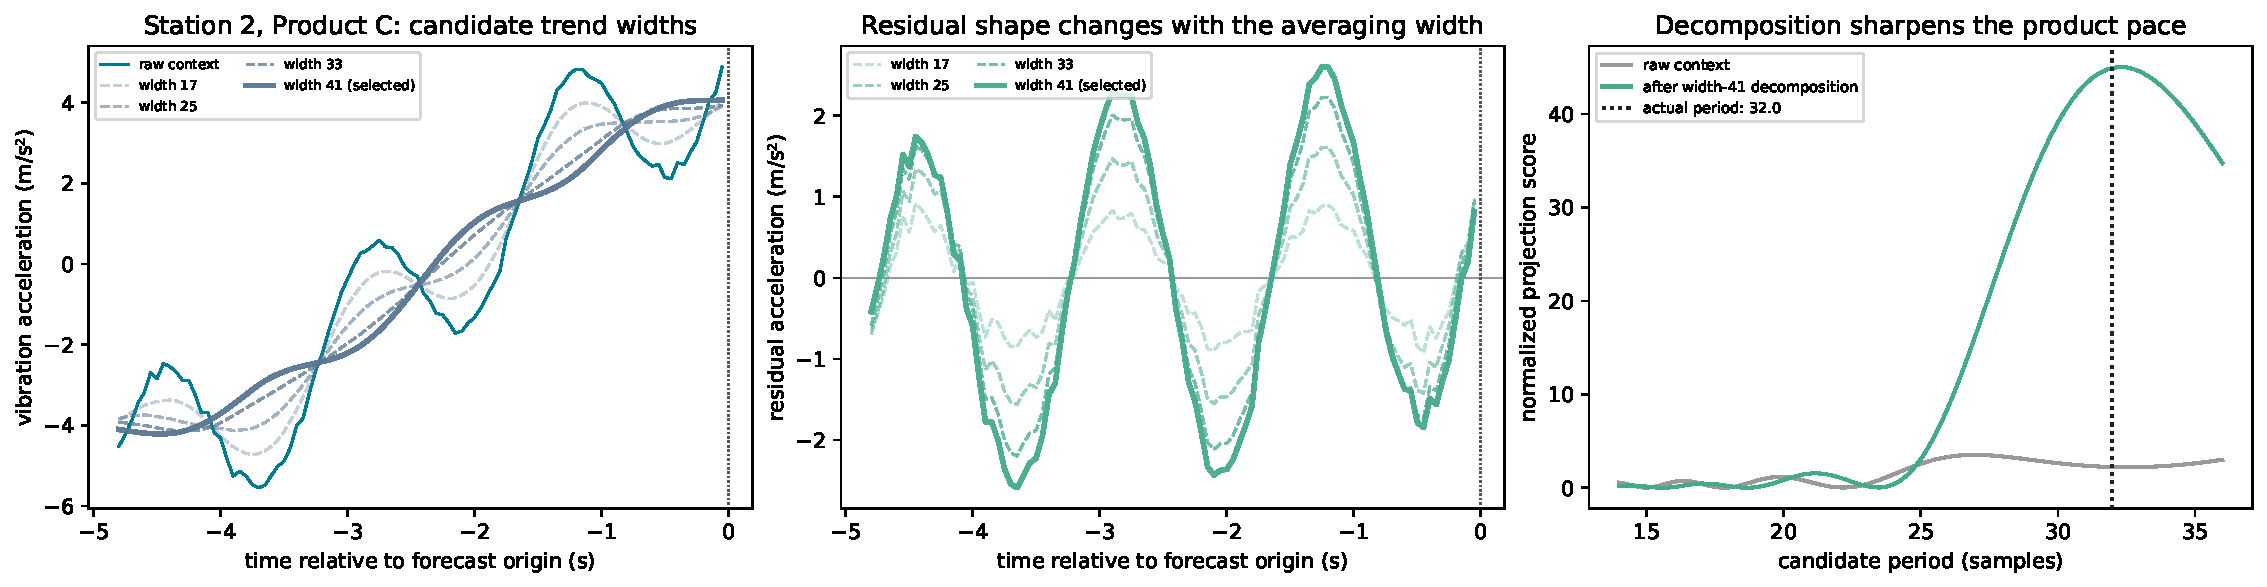
\includegraphics[width=0.95\linewidth]{figures/2.1-1.pdf}
\caption{Output 2.1: candidate trend widths, residuals and the period projection before and after width-41 decomposition.}\label{fig:o21}
\end{figure}

\subsection*{Response 3: mixing by temporal delay (Outputs 3.1, 3.2)}

\begin{itemize}
  \item \textbf{Checks.} Output 3.1 reproduces the direct circular correlation
        $[4,-4,4,-4]$ for $[1,3,1,3]$. The worked aggregation gives
        $z_0=\tfrac34 v_3+\tfrac14 v_1=35$, confirming position $t$ reads $t-\tau$.
  \item \textbf{Strongest recurrence (Output 3.2, validation window).} For station 2,
        Product A (actual period $P=16.13$), the residual correlation peaks at lags 16 and
        32, i.e.\ $P$ and $2P$ rounded to integers, with correlations 0.896 and 0.897, and
        again near 48 ($3P$, about 0.89). The troughs near 8, 24 and 40 are the
        half-period anti-alignments. Integer multiples appear because a shift by $kP$ also
        aligns peaks with peaks.
  \item \textbf{Why decomposition cleans the evidence.} On the raw context the curve
        falls from about 0.45 at lag 8 to about $-0.55$ near lag 40, with only a small
        plateau around lags 26 to 32 and no peak at 16 or 32. A rising ramp stays similar to itself after small shifts
        and dissimilar after large circular shifts (the wrap puts the high end next to
        the low end), so the drift dominates every lag. Removing $T$ leaves the
        oscillation, and lags that are multiples of $P$ then stand out by about 0.9. The
        delay mixer ranks delays by exactly this kind of score (on learned $q,k$), so it
        can only choose good delays if the slow part does not swamp the ranking.
  \item \textbf{Consequence in the models (Output 4.1).} The delay mixer alone gives the
        largest single gain (established RMSE 0.426 to 0.219) and delay + decomposition
        is best among neural models (0.199), consistent with this diagnostic.
  \item \textbf{Where the bias is wrong.} An isolated transient, such as a bearing knock
        or a jam that appears once in the context, has no recurrence. Circular delay
        scores spread its energy over many lags, top-$K$ selection then copies shifted
        versions of the transient into positions where it never happened, and the
        forecast either echoes a spurious repeat or averages it away. The same happens
        when the period drifts within the context, because no single delay aligns the
        early and late cycles.
\end{itemize}

% ---------------------------------------------------------------------------
\begin{figure}[h]\centering
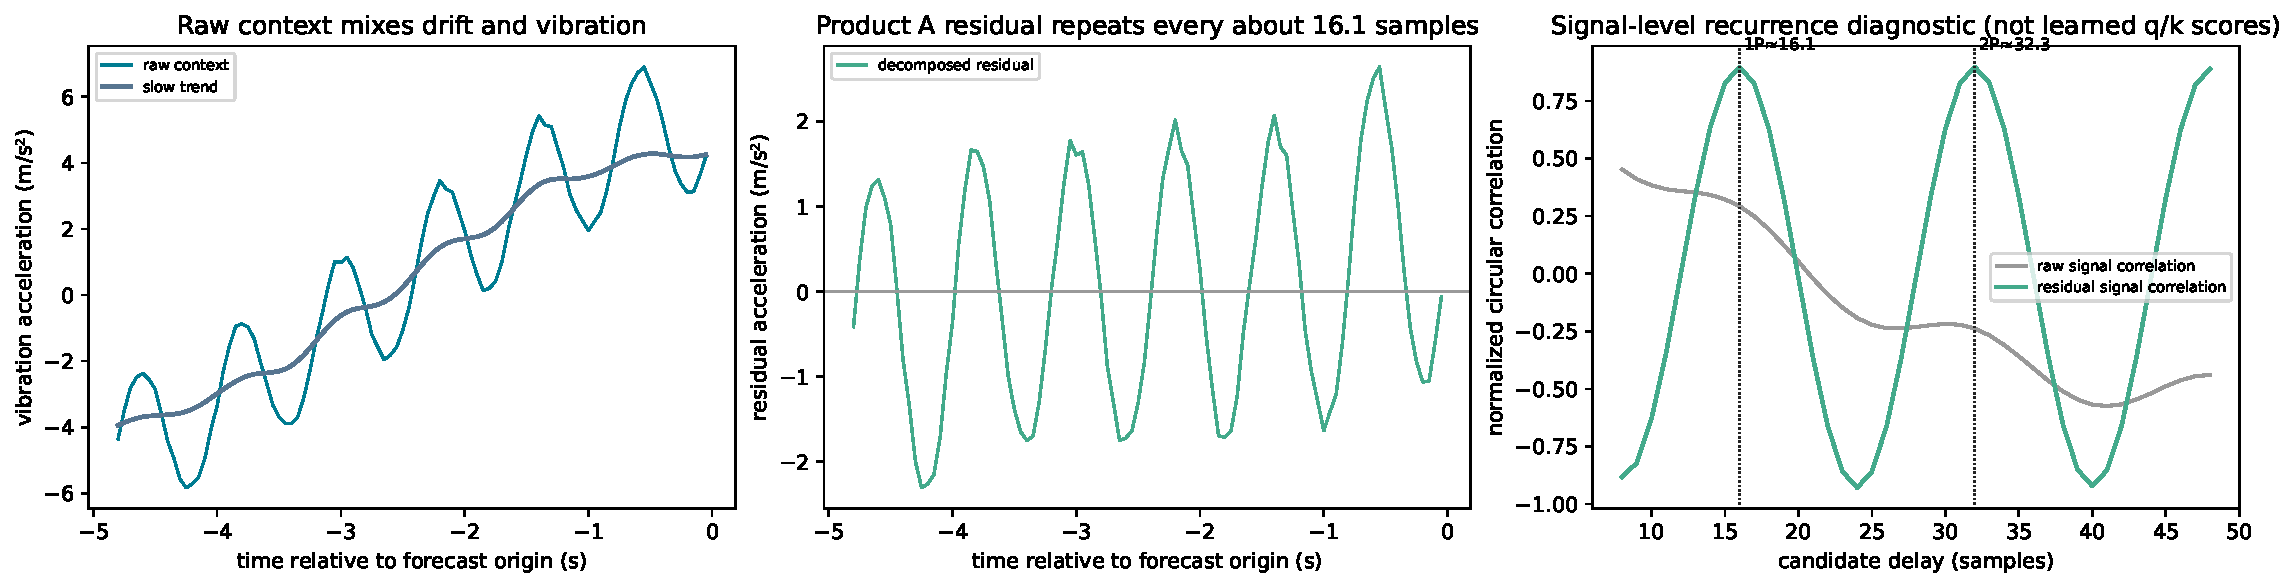
\includegraphics[width=0.95\linewidth]{figures/3.2-1.pdf}
\caption{Output 3.2: signal-level recurrence diagnostic (raw vs decomposed residual correlation), not learned q/k scores.}\label{fig:o32}
\end{figure}

\subsection*{Response 4: compare designs and deploy (Outputs 4.1--4.3)}

\textbf{(a) Prediction, written before Output 4.1.}
Decomposition should help most when the slow component is prominent, because it
removes the ramp before the mixer sees it and gives the trend its own linear head. The
delay mixer on raw input would rank delays by the ramp's self-similarity instead of the
vibration.

\textbf{(b) Validation errors, established stations (MSE in (m/s$^2$)$^2$).}

\begin{center}\small
\begin{tabular}{lccccr}
\toprule
Model & RMSE & MSE & Held-out RMSE & Held-out MSE & Params\\
\midrule
Shared ridge              & 0.767 & 0.588 & 0.876 & 0.767 & 4\,608\\
Sensor-specific ridge     & 0.768 & 0.590 & n/a   & n/a   & 13\,824\\
Period-routed ridge       & \textbf{0.166} & \textbf{0.028} & \textbf{0.173} & \textbf{0.030} & 59\,904\\
Raw Attention             & 0.426 & 0.182 & 0.607 & 0.369 & 368\,368\\
Raw delay mixer           & 0.219 & 0.048 & 0.342 & 0.117 & 368\,370\\
Attention + decomposition & 0.297 & 0.088 & 0.441 & 0.195 & 373\,024\\
Autoformer-inspired       & 0.199 & 0.039 & 0.239 & 0.057 & 373\,026\\
\bottomrule
\end{tabular}
\end{center}

% Interpretation below is limited to 200 words.
\textbf{Interpretation.} Both switches help on their own. On stations 1--3 (validation
MSE), decomposition lowers Raw Attention by 0.094 and delay mixing by 0.134. The
combined model gains 0.142, less than their sum (0.227), so the gains overlap rather
than stack. This is consistent with both switches exploiting the same drift-plus-cycle
structure, although the 2$\times$2 design cannot identify the cause. Station 4 shows
the same pattern (gains 0.174 and 0.252 alone, 0.311 combined). The switches are not
uniformly additive per window either: in Output 4.1's contrasting cases the combined
model cuts a station-4 Product B window from 1.386 to 0.189 but loses on a station-2
Product A window (0.353 vs 0.139 for the raw delay mixer). Along the horizon (Output
4.2, validation, stations 1--3), every model starts near 0.11--0.15 m/s$^2$ at step 1
and diverges afterwards. Raw Attention grows 3.5$\times$ by step 48 (0.151 to 0.525),
the Autoformer-inspired model only 1.7$\times$ (0.136 to 0.235). On station 4 the raw delay
mixer degrades sharply late in the horizon (0.635 at step 48), whereas the combined
model stays near 0.30 (station 4).

\textbf{(c) Deployment.} Period-routed ridge for \textbf{both} populations. It has the
lowest validation RMSE on stations 1--3 (0.166 vs 0.199 for the best neural model) and
on station 4 (0.173 vs 0.239), about 6$\times$ fewer parameters and a closed-form fit
in under 0.1 s instead of 1\,424 s. It needs no station identity, so it transfers to
station 4. Test results (Output 4.3) confirm the choice without being used for it:
0.161 on stations 1--3 and 0.183 on station 4.

\begin{figure}[h]\centering
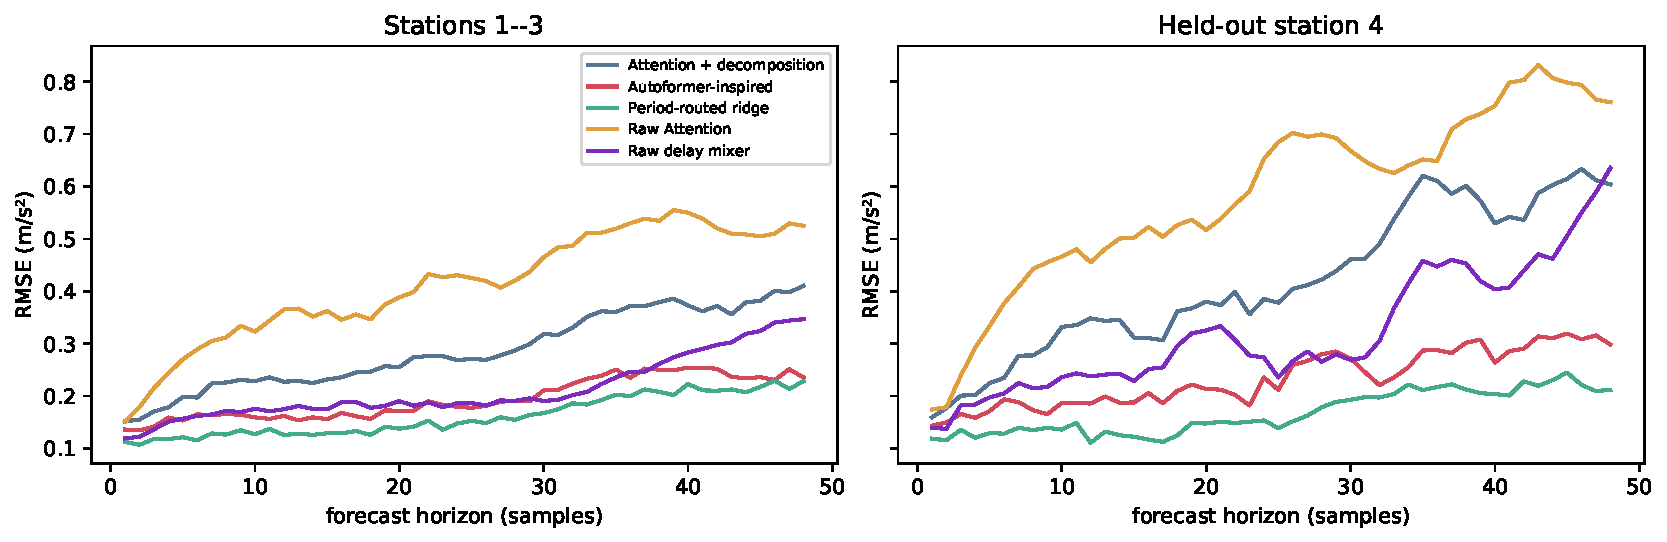
\includegraphics[width=0.95\linewidth]{figures/4.2-1.pdf}
\caption{Output 4.2: validation RMSE along the 48-step horizon, stations 1--3 (left) and station 4 (right).}\label{fig:o42}
\end{figure}

\clearpage
% Results are preserved in Question 2 - Leaderboard/results/ and submission_snapshots/.
\section{Task 2: Leaderboard Challenge}

\subsection{Data and forecasting setup}
The task is to forecast 168 values of an anonymised, non-negative physical quantity
from 43\,656 observed values. The original units, dates and identity are unavailable.
Ten optional external variables cover both the history and forecast horizon;
using their future values is explicitly permitted.
\begin{itemize}
  \item \textbf{Short memory and heavy tails.} Target autocorrelation is 0.97 at lag 1,
        0.40 at lag 24 and about 0.02 by lag 96. The median is 73, the 99th percentile
        418 and the maximum 994. Persistence alone is therefore unlikely to forecast
        the whole horizon well, and missing a few large peaks can dominate RMSE.
  \item \textbf{Recovered periodicity.} The spectrum and autocorrelation show a
        24-step cycle. I use index-derived sine/cosine features with periods 24 and
        8\,766. Interpreting these as daily and yearly cycles is an assumption,
        not something the anonymised timestamps establish.
  \item \textbf{Processing.} The target and continuous inputs are globally
        standardised using only the fit region. The non-negative variables D, E and F
        use $\log(1+x)$. Inputs include the ten optional variables, their trailing
        6- and 24-step means, and origin-relative marks ($h/168$ and $e^{-h/24}$).
        Trailing features use external data only; no future target enters an input.
\end{itemize}

\subsection{Chronological validation}
\begin{itemize}
  \item \textbf{Development split.} Fit on $[0,26304)$, early-stop on
        $[26304,35064)$ (origins every 24 steps), and compare designs on
        $[35088,43656)$: \textbf{51 non-overlapping 168-step blocks}.
        All blocks start at the same phase of the 24-step cycle as the hidden horizon.
  \item \textbf{Multiple seeds.} Each development configuration uses three seeds.
        Tables report seed mean and standard deviation unless identified as ensemble
        results. Paired block comparisons use the seed-averaged block errors.
        Seed spread is comparable to many design gains, so single runs are insufficient.
  \item \textbf{Second fold.} Later comparisons also fit on $[0,17520)$,
        early-stop on $[17520,26304)$ and evaluate the next 52 weekly blocks.
        The 16 edge weeks of the recent fold and 17 of the earlier fold are called
        \emph{winter-like} below, based on the assumed yearly cycle. Their errors are
        a useful stress test, but the season and hidden-week difficulty are uncertain.
  \item \textbf{Selection.} The first submission used full-holdout RMSE, with cost
        and edge-week performance as tie-breakers. Later changes were checked on both
        folds, seeking a mean weekly edge-error reduction of at least 3 RMSE and wins
        on at least 20 of 33 edge weeks. These development periods were reused during
        model selection, so they are not an untouched final test.
\end{itemize}

\subsection{Autoformer and initial design choices}
The encoder-decoder is written in \path{pa1q2/autoformer.py}.
It follows Wu et al. (2021), the public \path{thuml/Autoformer} implementation, and the delay-aggregation
convention from Task 1. It contains both required mechanisms:
\begin{itemize}
  \item \textbf{Progressive decomposition.} A centred moving average (kernel 25,
        replicate padding) separates trend and residual at the input and after every
        sublayer. Decoder trend contributions are accumulated through a projection.
  \item \textbf{Auto-Correlation.} FFT-based scores from learned queries and keys
        select $k=\lfloor\ln L\rfloor$ delays, followed by softmax-weighted circular
        aggregation of values. This replaces pointwise attention in encoder self,
        decoder self and decoder cross mixing.
  \item \textbf{Initial training.} Context 168, label length 48, horizon 168, one
        encoder and decoder layer, four heads, dropout 0.1, batch 64, gradient clip 1,
        MSE on the standardised raw target. Adam starts at $3\cdot10^{-4}$, halves
        each epoch, and stops with patience 2, at most six epochs. Final-model changes
        are specified in Section~\ref{sec:final}.
\end{itemize}

\subsection{Required optional-data ablation}
Three seeds per configuration, $d_\text{model}=32$; ES is early-stopping RMSE and
holdout covers 51 recent blocks.
\begin{center}\small
\begin{tabular}{lrrrrrr}
\toprule
Optional inputs & Params & ES RMSE & Holdout RMSE & MAE & sMAPE (\%) & Edge RMSE\\
\midrule
None                  & 21\,569 & 102.6 & 97.7 $\pm$ 2.8 & 72.2 & 74.9 & 119.4\\
Past only             & 27\,329 & 104.9 & 99.0 $\pm$ 0.9 & 72.2 & 78.6 & 119.9\\
Past + horizon        & 23\,489 & 79.2  & 74.4 $\pm$ 1.3 & 51.7 & 72.8 & 88.2\\
\bottomrule
\end{tabular}
\end{center}
Reference holdout RMSEs are
climatology 93.0, last-week mean 97.9, persistence 147.7, direct ridge without
covariates 87.7, and direct ridge with known-horizon covariates 71.5.
\begin{itemize}
  \item \textbf{Horizon values matter.} Known-horizon inputs reduce RMSE by 24\%
        (97.7 to 74.4), improve MAE and sMAPE, and beat the no-input model on 44 of 51
        blocks (paired sign test $p\approx10^{-7}$). The effect is much larger than
        the seed spread. External conditions during the forecast horizon carry useful
        information beyond the target history.
  \item \textbf{Past-only inputs did not help here.} Their 99.0 RMSE is close to
        97.7 without external data. This supports feeding the known horizon to the
        decoder, rather than relying on encoder history alone; it is not a claim that
        past covariates are generally useless.
\end{itemize}

\begin{figure}[h]\centering
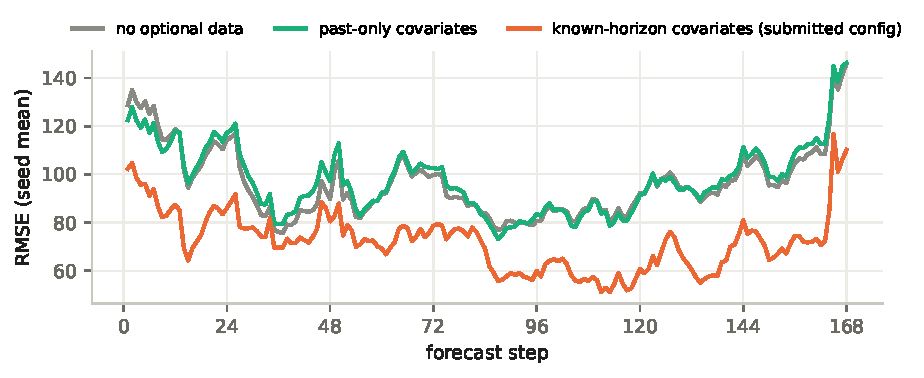
\includegraphics[width=0.49\linewidth]{figures/q2_horizon.pdf}\hfill
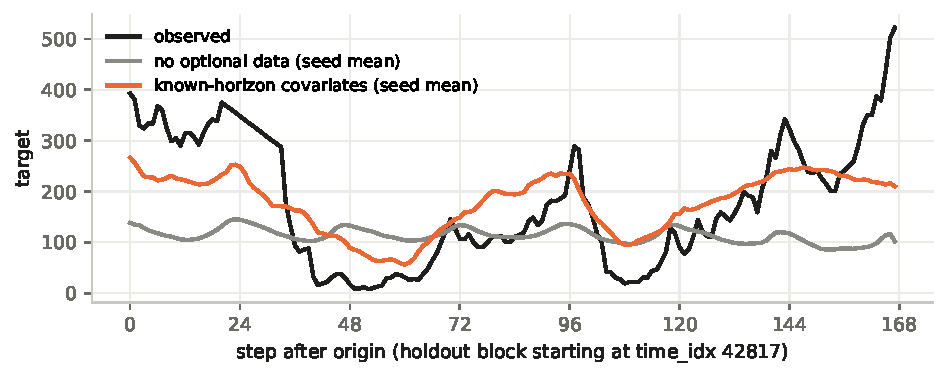
\includegraphics[width=0.49\linewidth]{figures/q2_example_week.pdf}
\caption{Left: per-step holdout RMSE (seed mean); the known-horizon model improves
every step. Right: an example from the most volatile late-year holdout week.}
\label{fig:q2horizon}
\end{figure}

\subsection{Which changes were worth keeping?}
\begin{center}\small
\begin{tabular}{lrrr}
\toprule
Initial variant (known-horizon inputs, three seeds) & Params & Holdout RMSE & Edge RMSE\\
\midrule
$d=32$ base                         & 23\,489 & 74.4 $\pm$ 1.3 & 88.2\\
$d=32$, $\log(1+y)$ target          & 23\,489 & 81.6 $\pm$ 10.4 & 88.2\\
$d=16$                              & 6\,625  & 75.1 $\pm$ 1.1 & 87.1\\
$d=16$, width-5 input embedding     & 10\,977 & 74.5 $\pm$ 2.6 & 85.5\\
\quad + horizon marks, no anchor   & 11\,297 & 73.2 $\pm$ 2.4 & 82.9\\
\quad + horizon marks and anchor   & 11\,297 & 72.9 $\pm$ 1.9 & 85.4\\
\bottomrule
\end{tabular}
\end{center}
\begin{itemize}
  \item \textbf{Raw target and a small model.} Log-target training improved MAE and
        sMAPE but under-predicted large peaks and gave unstable RMSE. Halving model
        width cost little measurable accuracy, so $d=16$ was preferable under the
        parameter/epoch penalty. More parameters or epochs alone did not establish
        a better model.
  \item \textbf{Horizon marks.} Origin-relative features explicitly identify the
        forecast step. Together with replicate padding they improved boundary errors
        and holdout RMSE. Anchoring was a close comparison (72.9 versus 73.2), so the
        anchored configuration was used for attempt 1, rather than claimed as a
        decisive improvement.
  \item \textbf{Negative results.} Refitting on more history, wider decomposition,
        extra rolling features, winter-weighted loss and square-root targets did not
        consistently improve edge weeks. A 27-model mixture improved recent-fold
        RMSE only from 69.3 to 68.1, at $P=345\,435$, $E=122$; it was not submitted.
        Full records remain in the repository.
\end{itemize}

\textbf{A more direct path for horizon inputs.} A covariate-only gradient-boosting
baseline scored 57.0 overall and 70.5 on recent edge weeks, against 69.3 and 82.0 for
the attempt-1 ensemble. This suggested that the horizon inputs held signal the
sequence model was not fully using. One possible explanation is smoothing inside
the decomposition/mixing path, but this mechanism was not isolated experimentally.
I compared a nonlinear covariate embedding with an additive per-step covariate head:
\begin{center}\small
\begin{tabular}{llrrr}
\toprule
Fold & Three-seed ensemble & All-week RMSE & Edge RMSE & Edge weeks won\\
\midrule
Recent  & Attempt-1 configuration & 69.34 & 81.97 & --\\
        & Covariate embedding MLP & 64.79 & 76.80 & 8/16\\
        & Direct covariate head   & 61.68 & 74.97 & 12/16\\
Earlier & Attempt-1 configuration & 77.43 & 106.13 & --\\
        & Covariate embedding MLP & 74.36 & 102.48 & 12/17\\
        & Direct covariate head   & 66.40 & 91.63 & 12/17\\
\bottomrule
\end{tabular}
\end{center}
Wins are relative to attempt 1 on the same blocks. The direct-head configuration
reduced mean weekly edge RMSE by 8.3 and won 24 of 33 weeks across both folds.
It also removes anchoring and changes the learning-rate schedule; these results
support the combined configuration, not the head's isolated contribution.

\subsection{Leaderboard results}
\begin{center}\small
\begin{tabular}{clrrrrr}
\toprule
Attempt & Model (three members) & RMSE & MAE & sMAPE (\%) & $P$ & $E$\\
\midrule
1 & Anchored Autoformer     & 81.56 & 60.96 & 57.81 & 33\,891 & 15\\
2 & Covariate embedding MLP & 81.93 & 62.75 & 59.58 & 38\,979 & 16\\
3 & Direct covariate head   & \textbf{62.95} & \textbf{46.31} & \textbf{49.63} & 53\,670 & 20\\
\bottomrule
\end{tabular}
\end{center}
\begin{itemize}
  \item Attempt 1 ranked fourth when submitted. Its 69.34 historical ensemble RMSE
        did not predict the hidden-week result. Edge-week RMSE of 81.97 was closer,
        consistent with seasonal difficulty, but neither estimate guarantees a rank.
  \item Attempt 2 improved historical validation in both folds but did not improve
        the scored week. A single 168-step block can disagree with a multi-block
        estimate, especially for a heavy-tailed series.
  \item Attempt 3 scored 62.96 after the efficiency penalty and ranked first at the
        time (previous best 69.16). RMSE was 23\% below attempt 1. This is a reported
        result, not a guarantee about later rankings or other weeks. Leaderboard
        feedback prompted further historical checks; candidate selection used those
        checks and early stopping, not access to hidden targets.
\end{itemize}

\subsection{Final submitted model (attempt 3)}\label{sec:final}
\begin{itemize}
  \item \textbf{Architecture.} Autoformer with $L=168$, label length 48,
        \texttt{pred\_len}=168, one encoder and decoder layer, $d_\text{model}=16$,
        four heads, $d_\text{ff}=32$, kernel 25, dropout 0.1, width-5 covariate
        embedding, replicate padding and horizon marks. A direct head
        ($36\to64\to64\to1$, GELU) maps each step's known inputs to an additive
        forecast correction. Decomposition and all three Auto-Correlation mixers
        remain present. There is no last-value anchoring.
  \item \textbf{Training and selection.} Fit on $[0,35064)$ and early-stop on the
        51 recent blocks, with Adam at $10^{-3}$ decayed by 0.8 per epoch, patience 3,
        at most ten epochs, batch 64, MSE and gradient clip 1. Of seven seeds (0--6),
        seeds 2, 3 and 4 form the final ensemble, selected using the early-stopping
        set. Their best RMSEs are 59.7, 65.8 and 63.7, at epochs 4, 4 and 3.
        Seeds 0, 1 and 6 stopped at RMSE 81--83; seed 5 was also excluded to keep
        the ensemble at three members. Selection adds uncertainty beyond an
        unselected three-seed comparison.
  \item \textbf{Forecast and cost.} Each member's forecast is floored at 7.0 (the
        fit-region target's 1st percentile), then the three forecasts are averaged.
        The 168 outputs cover \texttt{time\_idx} 43\,657--43\,824 in order.
        $P=3\times17\,890=53\,670$ and $E=7+7+6=20$, including patience epochs;
        there was no full-history refit. Four discarded runs used a further 17 epochs,
        disclosed here but excluded from the submitted members' total.
  \item \textbf{Reproduction.} The \path{submission/} folder holds the forecasts
        and declaration. The declaration records all member arguments and epoch counts.
        \texttt{pa1q2.submission} reloads weights and checks parameter counts.
        Training/export commands are in the Task 2 README. Final snapshot:\\
        \path{submission_snapshots/covhead_s2_s3_s4_2026-09-29/}.
\end{itemize}

\textbf{Limits and takeaway.} The final comparison changes the covariate head,
anchoring and schedule together. It does not prove that smoothing caused the earlier
errors. Development blocks were reused, the final members were selected on early
stopping, and the hidden score covers only one week. The strongest finding is the
large benefit of known-horizon inputs in the required multi-seed ablation. The final
configuration makes better use of those inputs while keeping the Autoformer mechanisms.

\clearpage
\begin{figure}[ht]\centering
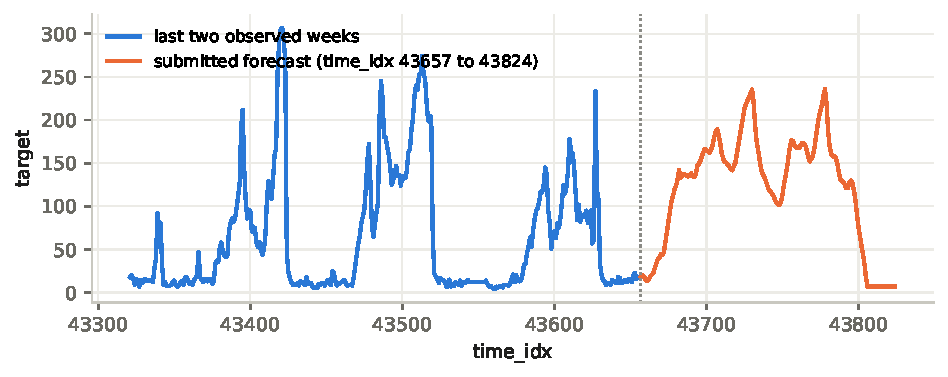
\includegraphics[width=0.74\linewidth]{figures/q2_final_forecast.pdf}\\[4pt]
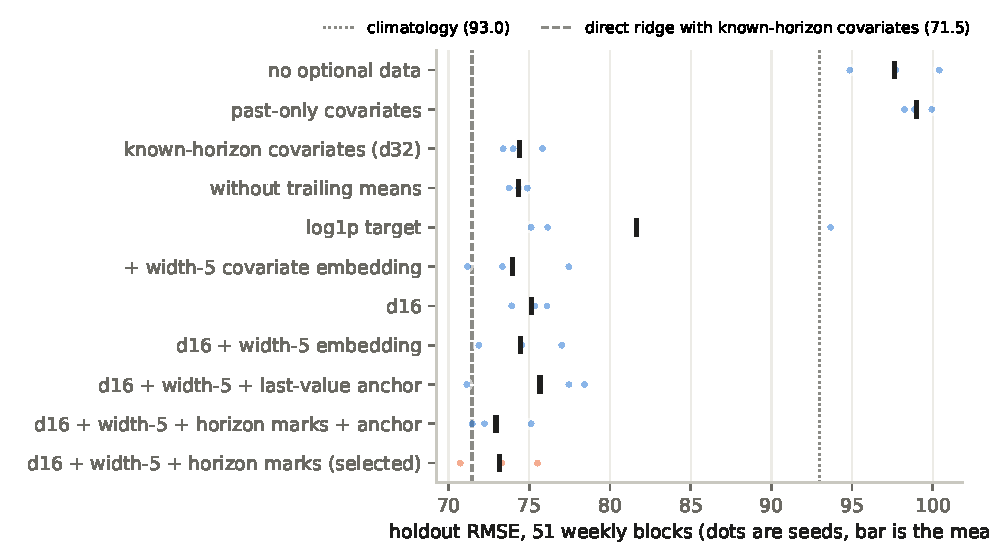
\includegraphics[width=0.95\linewidth]{figures/q2_ablation.pdf}
\caption{Top: last two observed weeks and the attempt-3 forecast. Bottom: initial
ablation runs on 51 holdout blocks (dots are seeds, bars are means); reference lines
show climatology and covariate ridge. The initial selected row refers to attempt 1.}
\label{fig:q2final}
\end{figure}

\subsection{Short reflections}
The direct 168-step output avoids feeding forecast errors back into the model,
although horizon errors can remain correlated. Global scaling preserves absolute
level; restoring a window's level after relative normalisation would not by itself
let the network condition on that level. Known-horizon inputs belong in the forecast
path, as the optional-data ablation demonstrates. Integer indices allow recovered
phase features on this regular grid, but they do not establish weekdays, holidays
or a real calendar; the yearly interpretation remains an assumption.

\clearpage
\section*{Generative AI use}
I used Claude (Anthropic) and OpenAI Codex as assistants for this assignment.

\textbf{Prompts.}
\begin{itemize}
  \item I asked Claude to read the PA1 handout and notebook, complete the required
        implementation cells, run the notebook on the full preset, and draft the Task 1
        responses from the numbered outputs.
  \item I asked Claude to build a small Autoformer solution for the leaderboard task,
        including preprocessing, chronological validation, optional-data ablation,
        multi-seed runs, plots, and the final 168-value submission string.
  \item I asked Codex to review Claude's work against the assignment requirements,
        check for over-engineering or non-student-like writing, verify the leaderboard
        submission files, and make the final report submission-ready.
\end{itemize}

\textbf{What the assistant produced.}
\begin{itemize}
  \item Task 1: the three notebook implementations, the full-preset run, and first drafts
        of Responses 1A--4 from the exported Outputs.
  \item Task 2: the \texttt{pa1q2} package (data handling, from-scratch Autoformer,
        training with resumable early stopping, baselines, aggregation, figures,
        submission writer), the experiment plan and runs, and a first draft of this
        section.
  \item Final review: checks for missing fields, exact prediction count, declared
        parameter and epoch values, and consistency between the report and saved outputs.
\end{itemize}

\textbf{My edits and checks.}
\begin{itemize}
  \item I checked the notebook outputs, kept the full-preset figures and tables, and
        edited the responses to focus on the required comparisons instead of only
        describing the code.
  \item For Task 2, I used my own validation split to choose the final model, kept the
        optional-data ablation, and did not use the public leaderboard as a validation
        signal.
  \item I verified that \texttt{submission/predictions.txt} contains exactly 168 values
        in chronological order and that the declared parameter count and epoch count
        match the saved final run.
\end{itemize}


\section*{References}
\begin{itemize}
\item Wu, Xu, Wang, Long (2021). Autoformer: Decomposition Transformers with Auto-Correlation
for Long-Term Series Forecasting. NeurIPS. Reference code: \url{https://github.com/thuml/Autoformer}.
\item Vaswani et al.\ (2017). Attention Is All You Need.
\item Zeng et al.\ (2023). Are Transformers Effective for Time Series Forecasting?
\item Hyndman and Athanasopoulos. Forecasting: Principles and Practice.
\end{itemize}
\end{document}
